\documentclass{article}

% Encoding and Geometry
\usepackage[utf8]{inputenc}
\usepackage[a4paper, margin=1in]{geometry} % Standard 1-inch margins for better layout
\usepackage{parskip}

% Math Packages
\usepackage{amsmath, amsfonts, mathtools}

% Graphics and Figures
\usepackage{graphicx}
\usepackage{caption}
\usepackage{subcaption}
\usepackage{multirow}
\usepackage{tikz}
\usetikzlibrary{positioning} % Ensures compatibility with Overleaf

% Hyperlinks
\usepackage[colorlinks=true, linkcolor=blue, urlcolor=blue]{hyperref} % Load last to avoid conflicts

% Floating Objects Placement
\usepackage[section]{placeins} 

% Bibliography
\usepackage[
    backend=biber,
    style=alphabetic,
    sorting=ynt
]{biblatex}
\addbibresource{references.bib}

% Title Information
\title{Maglev White Paper}
\author{Euler Labs}  % Optionally add an author here
\date{February 2025}

\begin{document}

\maketitle

\begin{abstract}    
    Maglev is an Automated Market Maker (AMM) that uses unique features of Euler lending vaults to dramatically \textbf{mag}nify capital efficiency using \textbf{lev}erage. Unlike traditional AMMs that require fragmented liquidity pools, Maglev enables a single, cross-collateralized vault to provide liquidity across multiple asset pairs simultaneously, maximizing capital efficiency and scaling liquidity across DeFi. Using the Ethereum Vault Connector (EVC), Maglev allows market makers to borrow the out token of a swap using the in token as collateral, unlocking deep liquidity without requiring large static deposits. This liquidity-sharing model allows Maglev to achieve up to 40x the liquidity depth of traditional AMMs, efficiently repurposing idle assets for optimal capital utilization. At the core of Maglev is a highly customizable AMM curve that governs swap exchange rates, ensuring deep, just-in-time liquidity while dynamically incentivizing market balance. By combining on-demand borrowing, shared liquidity, and flexible AMM mechanics, Maglev eliminates inefficiencies in existing liquidity provisioning, offering superior depth, reduced costs, and greater control for liquidity providers.
\end{abstract}

\section{Introduction}

Maglev enhances trade execution by increasing the size of swaps that can be serviced compared to traditional AMMs. This is made possible by combining a novel AMM curve with the advanced \href{https://docs.euler.finance/developers/evc/keyConcepts?_highlight=operator#batch-operations}{check deferrals} and \href{https://docs.euler.finance/developers/evc/keyConcepts?_highlight=operator#operators}{operator} features of the Ethereum Vault Connector (EVC). Market makers supply an initial amount of liquidity to a `swap account' which can then be amplified through borrowing. Specifically, when a user swaps an `in token,' Maglev borrows the corresponding `out token,' using the `in token' as collateral. Later, when a swap occurs in the reverse direction, the incoming `in token' repays the outstanding loan, and any excess collateral is returned as the `out token,' effectively closing the position. This leveraged approach significantly increases the available liquidity provided by Maglev and multiplies swap fees. It is somewhat analogous to MEV bots that provide just-in-time single-tick liquidity to Uniswap v3 in order to capture fees on large trades.

Beyond individual swap accounts, Maglev takes capital efficiency further by taking advantage of Euler's modular design to allow multiple swap accounts to be built on top of the same lending vaults. This means that the same idle liquidity inside a single vault can provide depth for swaps across multiple asset pairs simultaneously. Much like Curve’s 3pool, but generalized to any number of asset pairings, a USDC vault could provide deep liquidity for 10+ correlated assets without requiring separate liquidity pools for each.

Maglev’s exchange rates are governed by a highly customisable AMM curve (illustrated in Figure \ref{fig:fig1}) which incentivises swappers to maintain market maker positions in balance over time. The Maglev AMM curve is a novel construction blending constant-sum and constant-product models, allowing swap account creators to tailor their AMM parameters. Like \href{https://berkeley-defi.github.io/assets/material/StableSwap.pdf}{Stableswap}, it supports concentrated liquidity for correlated assets, as well as \href{https://app.uniswap.org/whitepaper.pdf}{Uniswap v2}-style distributed liquidity for uncorrelated pairs. However, unlike those more traditional AMMs, Maglev allows asymmetric liquidity deposits, where different amounts of liquidity can be added to each side of the pool, and single-sided liquidity concentration, enabling deeper concentration of liquidity on one side of the pool relative to the other. This enables it to simulate the behaviour of atypical AMM protocols, like the MakerDAO \href{https://mips.makerdao.com/mips/details/MIP29}{Peg Stability Module} (PSM).

For end-users, Maglev functions like a typical Uniswap-style interface. However, behind the scenes, it incorporates advanced mechanisms such as borrowing and repaying, custom pricing curves, and dynamic liquidity provisioning. The main target audience for liquidity providers in Maglev AMMs are professional market makers, token issuers, and other DAOs, whilst the main target audience for swappers are leverage traders on Euler, aggregators, intent solvers, and MEV bots.  

\section{Example}

Suppose that Euler allows borrowing of USDT with USDC as collateral at a loan-to-value (LTV) ratio of 0.95, and vice versa. This means that for every \$1 of USDC or USDT collateral, a user can borrow up to \$0.95 of the other asset. 

Now suppose you have a swap account with 1M USDC deposited as initial liquidity. Using maximum leverage your account could support deposits of 20M USDC and debts of 19M USDT. Alternatively, if you swapped your 1 million USDC to 1 million USDT, it could support the opposite. Let’s say another user wants to swap 10M USDC for USDT. The steps are as follows:

\begin{enumerate}
    \item They send 10M USDC to your swap account as the swap input.
    \item Your swap account deposits the 10M USDC as collateral in Euler.
    \item Your swap account borrows approximately 10M USDT against the account's collateral, which includes your original deposit, alongside the swap input.
    \item It sends the borrowed USDT to the user as the swap output.
\end{enumerate}

\quad
Importantly, this isn’t a 1:1 swap because: a) you charge a fee for facilitating the swap; and b) the exact swap output is determined by an AMM curve, which factors in increasingly large price impact as the swap input amount increases. After the swap, your swap account now holds 11M USDC deposits and 10M USDT debt. It earns interest on the supplied USDC but must also pay interest on the borrowed USDT.

Later, when a swap occurs in the reverse direction, the incoming `in token' repays the outstanding loan, and any excess collateral is returned as the `out token.' The AMM curve dynamically adjusts incentives such that imbalances encourage swaps in the opposite direction, facilitating natural rebalancing. This mechanism ensures that positions do not remain open for extended periods, reducing exposure to borrowing costs. Over time, you will incur costs due to small interest rate differentials, whilst generating significant swap fees through utilisation of idle liquidity in the lending protocol. The whole process is depicted in Fig. \ref{fig:maglev_liquidity}.

\bigskip
\begin{figure}[h]
    \centering
    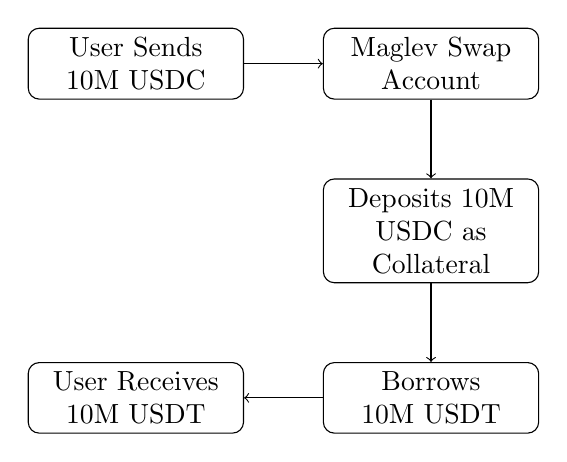
\begin{tikzpicture}[
        node distance=1cm, 
        every node/.style={draw, text width=2.5cm, align=center, rounded corners}
        ]
        % Nodes
        \node (user1) {User Sends 10M USDC};
        \node (maglev) [right=of user1] {Maglev Swap Account};
        \node (deposit) [below=of maglev] {Deposits 10M USDC as Collateral};
        \node (borrow) [below=of deposit] {Borrows ~10M USDT};
        \node (user2) [left=of borrow] {User Receives 10M USDT};
        
        % Arrows
        \draw[->] (user1) -- (maglev);
        \draw[->] (maglev) -- (deposit);
        \draw[->] (deposit) -- (borrow);
        \draw[->] (borrow) -- (user2);
    \end{tikzpicture}
    \caption{\textbf{Swap flow in Maglev AMM}. Maglev’s just-in-time liquidity borrowing. The swap account dynamically increases liquidity by borrowing the ``out token" against the ``in token."}
    \label{fig:maglev_liquidity}
\end{figure}

\section{Curve}

The space of possible reserves in a Maglev AMM is determined by how much debt a swap account is allowed to hold. The Maglev curve passes through an equilibrium point $(x_0, y_0)$, at which the marginal price is defined by:

\begin{equation}
\frac{dy}{dx} \Big|_{(x_0, y_0)} = -\frac{p_x}{p_y}.
\end{equation}

Unlike most AMM curves, which are usually defined by a single convex function, Maglev uses a piecewise-defined curve, with different functions providing trading behaviour either side of the equilibrium point:

\begin{equation}
    \label{eq:fx-main}
    f(x) =
    \begin{dcases}
        f_1(x), 
        & 0 < x \leq x_0 \\
        f_2(x), 
        & x_0 < x
    \end{dcases}.
\end{equation}

In the domain $0 < x \leq x_0$, the curve is defined by

\begin{equation}
    \label{eq:fx1-main}
    f_1(x) 
    =
    y_{0}+\frac{p_{x}}{p_{y}}\left(x_{0}-x\right)\left(c_{x}+\left(1-c_{x}\right)\left(\frac{x_{0}}{x}\right)\right).
\end{equation}

In the domain $x_0 < x$, the curve is defined by

\begin{equation}
    \label{eq:fx2-main}
    f_2(x) 
    =
    \frac{
        \sqrt{
            \left( \frac{p_x}{p_y} (x - x_0) + y_0 (1 - 2c_y) \right)^2 
            + 4c_y (1 - c_y) y_0^2
        } 
        - \left( \frac{p_x}{p_y} (x - x_0) + y_0 (1 - 2c_y) \right)
    }{2c_y}.
\end{equation}

 The curve coefficients in these equations, \( c_x, c_y \in [0, 1] \), represent liquidity concentration parameters, determining how steeply the curve slopes to the left and right of the equilibrium point $(x_0, y_0)$. When \( c_x, c_y \) are close to 1, the curve behaves more like a constant-sum AMM, while for values close to 0, it behaves more like a constant-product AMM. A full derivation is given in the Appendix \ref{sec:curve-derivation}.  
 
 \begin{figure}[h]  % 'h' places it here, 't' for top, 'b' for bottom, 'p' for separate page
    \centering  % Centers the image
    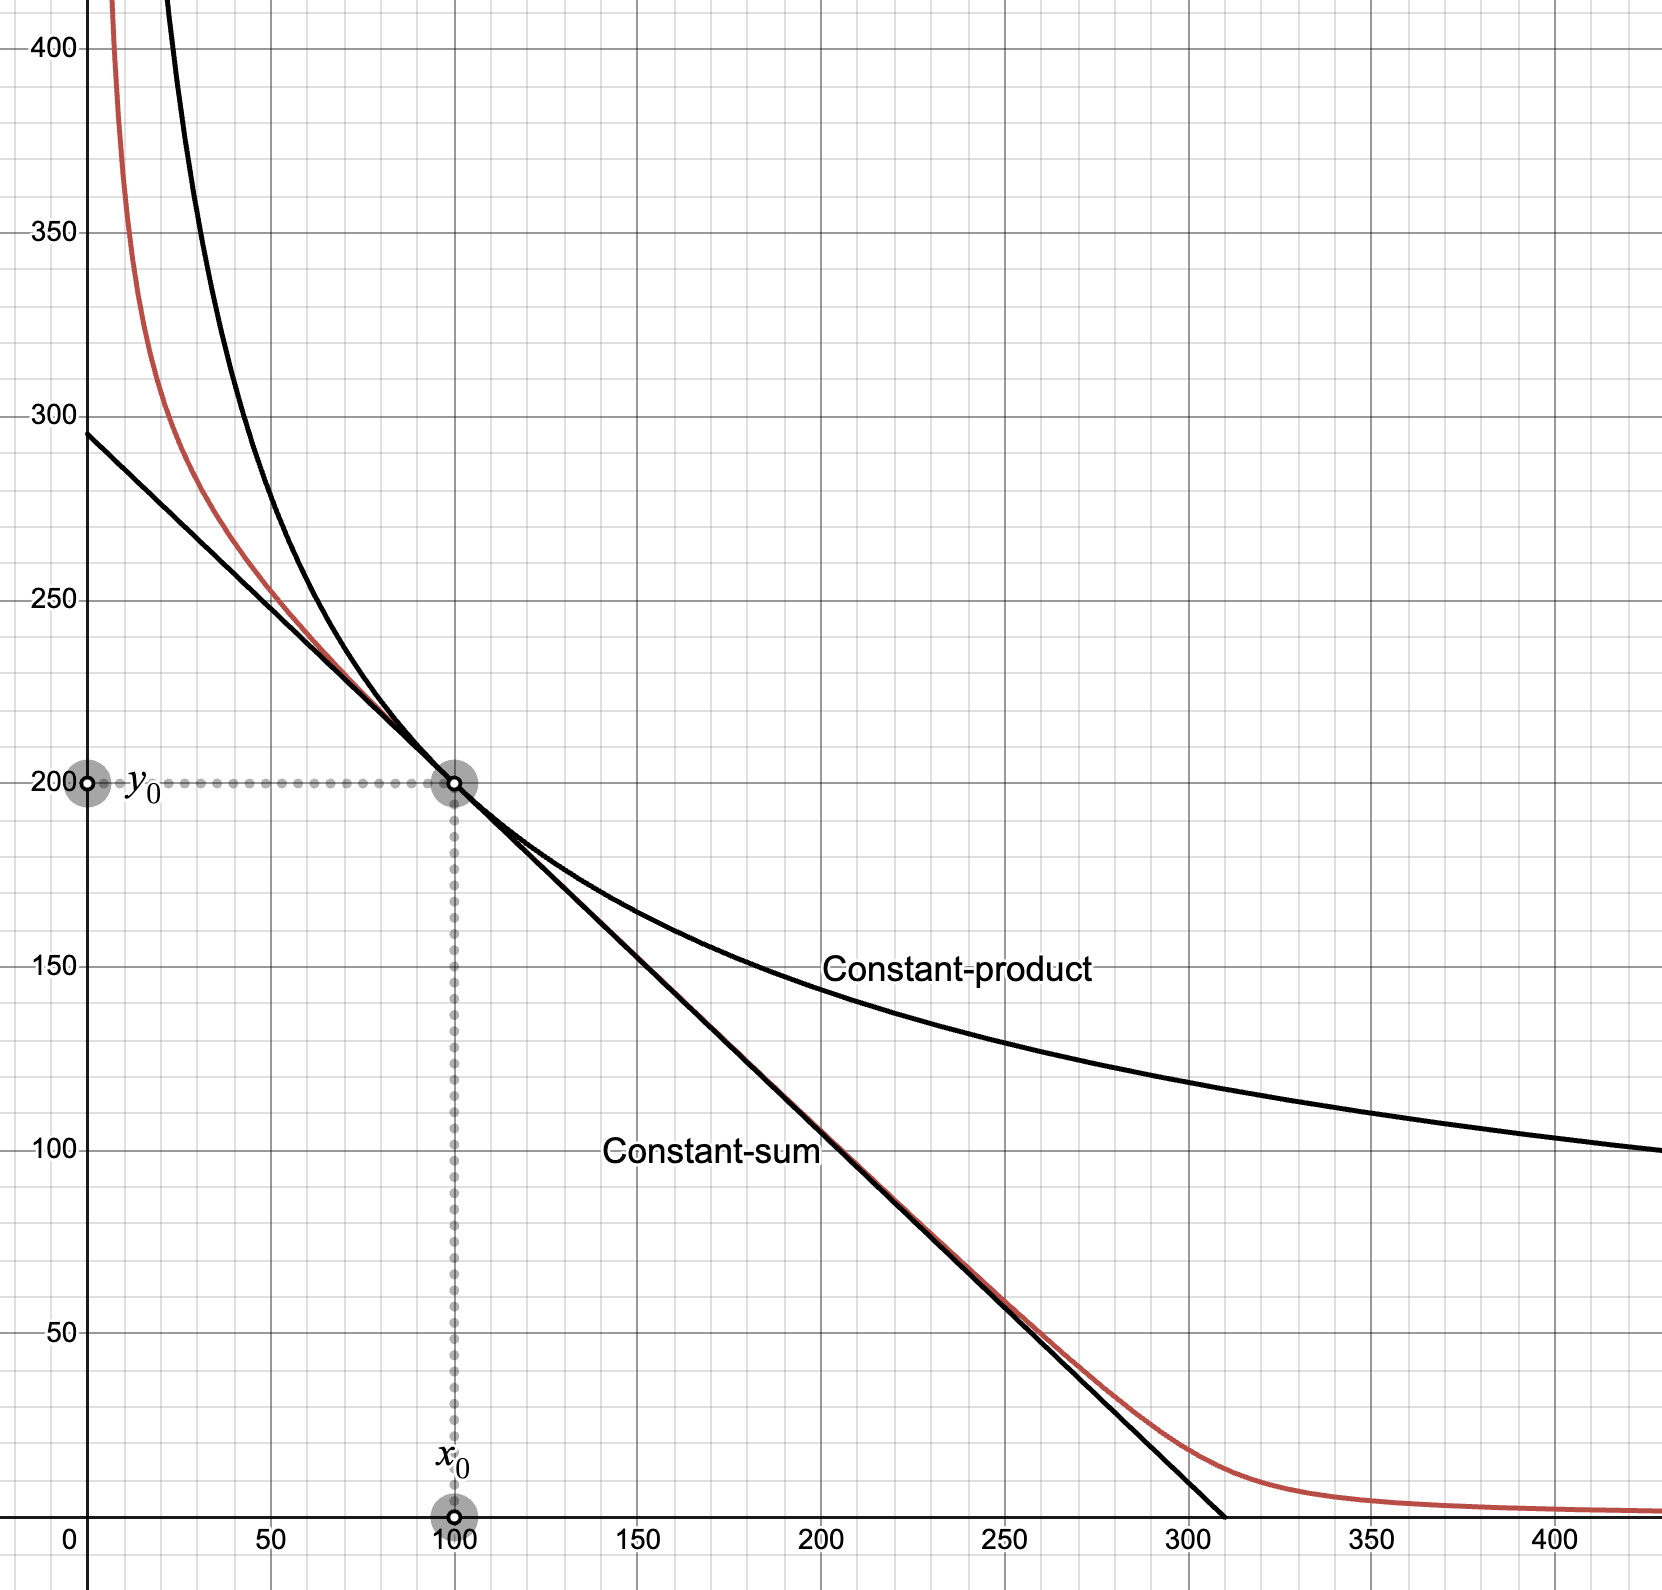
\includegraphics[width=0.5\textwidth]{curve.png} % Adjust width as needed
    \caption{\textbf{Maglev AMM curve.} The Maglev curve (red line) consists of two sides with separate reserve values $x_0, y_0$ and concentration parameters $c_x, c_y$, allowing liquidity to be distributed asymmetrically. This means liquidity can be more or less dense or concentrated on one side of the AMM relative to the other. The exchange rate at equilibrium is determined by the pricing parameters $p_x, p_y$ and is fully flexible. You can interact with the curve \href{https://www.desmos.com/calculator/gzwmvbs1dk}{here} on Desmos to compare its behavior with traditional constant-sum and constant-product curves (black lines).}
    \label{fig:fig1}  % Useful for referencing the figure in text
\end{figure}

\section{Conclusion}

Maglev enhances Automated Market Making by leveraging just-in-time borrowing to expand liquidity depth dynamically. By integrating Euler’s lending vaults, it enables market makers to amplify positions efficiently while offering a customizable AMM curve that supports concentrated, distributed, and asymmetric liquidity structures. These features make Maglev adaptable to a wide range of trading strategies. However, this efficiency is not without some trade-offs. Swap accounts incur interest costs on borrowed assets, which can erode profitability if not offset by swap fees, interest on collateral, or token incentives. Additionally, Maglev inherits Euler’s risk parameters, making it most effective for correlated asset pairs with high loan-to-value (LTV) ratios, while volatile assets pose higher liquidation risks if positions become imbalanced. Despite these trade-offs, Maglev represents a breakthrough in AMM design by repurposing idle liquidity in lending protocols, reducing capital inefficiencies, and optimizing swap execution. By catering to professional market makers, DAOs, and algorithmic traders, it positions itself as a powerful tool for on-chain liquidity optimization.

\section*{Acknowledgments}

During a security review of Maglev, Chris Michel noted similarities between some of its underlying concepts and BlackHoleSwap, a project prototype he had reviewed years earlier. While Maglev was designed independently and without influence from that project, the resemblance is significant enough to warrant its recognition here as prior art.

\newpage
\section{Appendix}

\subsection{Curve derivation}
\label{sec:curve-derivation}

We start with an AMM containing reserves (initial liquidity) of two assets, \( x_0 \) and \( y_0 \), and define two standard AMM curve models.

\subsubsection{Constant-sum and constant-product AMM curves}

The constant-sum and constant-product AMM curves are given by:

\begin{align}
    x + y &= x_0 + y_0, \\
    xy &= x_0 y_0.
\end{align}

These curves intersect at the point \( (x_0, y_0) \), where their slope is:

\[
\frac{dy}{dx} \Big|_{(x_0, y_0)} = -1.
\]

To introduce arbitrary pricing, we extend these curves by adding pricing parameters \( p_x \) and \( p_y \).

\subsubsection{Generalising to arbitrary pricing}

We define new AMM equations incorporating custom pricing:

\begin{align}
    p_x x + p_y y &= p_x x_0 + p_y y_0, \\
    \label{eq:exponential-form}
    x^{p_y y_0} y^{p_x x_0} &= x_0^{p_y y_0} y_0^{p_x x_0}.
\end{align}

Taking the derivatives of these equations with respect to \( x \), we obtain:

\begin{align}
    \frac{dy}{dx} &= -\frac{p_x}{p_y}, \\
    \frac{dy}{dx} &= -\frac{p_x}{p_y} \frac{x_0 y}{y_0 x}.
\end{align}

These results confirm that at equilibrium \( (x_0, y_0) \), the slope is:

\[
\frac{dy}{dx} \Big|_{(x_0, y_0)} = -\frac{p_x}{p_y}.
\]

However, equation \eqref{eq:exponential-form} involves an exponential form, which makes it difficult to evaluate numerically. To resolve this, we introduce the concept of virtual reserves.

\subsubsection{Introducing virtual reserves for simplicity}

Note that in the interval $0 < x < x_0$ trading should not depend on the initial amount of $y_0$ liquidity. Swaps from should only increase liquidity beyond $y_0$ and deplete the $x_0$ liquidity. This suggests that we can split the domain of the AMM curves into two, and replace the real reserve $y_0$ in the interval $0 < x < x_0$ with an idealised virtual reserve $y_v$. Using the equilibrium condition:

\[
p_x x_0 = p_y y_0,
\]

we derive:

\[
y_v = x_0 \frac{p_x}{p_y}.
\]

Substituting into our pricing equations and simplifying, we obtain two modified AMM equations:

\begin{align}
    y &= \frac{p_x}{p_y} (2x_0 - x), \\
    y &= \frac{p_x}{p_y} \frac{x_0^2}{x}.
\end{align}

Since these curves no longer pass through \( (x_0, y_0) \), we correct them by adding back the difference \( y_0 - p_x / p_y x_0 \), leading to:

\begin{align}
    y &= y_0 + \frac{p_x}{p_y} (x_0 - x), \\
    y &= y_0 + \frac{p_x}{p_y} (x_0 - x) \left( \frac{x_0}{x} \right).
\end{align}

\subsubsection{Unifying into a single curve}

To create a single unified curve, we introduce a liquidity concentration parameter \( c_x \), which determines the curve’s behavior:

\begin{itemize}
    \item When \( c_x = 1 \), the AMM functions as a constant-sum model.
    \item When \( c_x = 0 \), the AMM behaves as a standard constant-product AMM.
    \item Intermediate values of \( c_x \) create a hybrid liquidity curve.
\end{itemize}

This gives the final equation:

\begin{equation}
    \label{eq:maglev-1}
    y = y_0 + \frac{p_x}{p_y} (x_0 - x) \left( c_x + (1 - c_x) \left(\frac{x_0}{x}\right) \right).
\end{equation}

This is equivalent to the function \( f_1(x) \) given by equation \eqref{eq:fx1-main} in the main text.

\subsubsection{Extending the curve to the \( x > x_0 \) region}

For \( x > x_0 \), we construct a reflected curve that also passes through \( (x_0, y_0) \) and maintains the required derivative:

\begin{equation}
    \label{eq:maglev-3-inverse}
    x = x_0 + \frac{p_y}{p_x} (y_0 - y) \left( c_y + (1 - c_y) \left(\frac{y_0}{y}\right) \right).
\end{equation}

Since this equation defines \( x \) in terms of \( y \), we invert it by solving for \( y \), leading to the quadratic equation:

\begin{equation}
    y = c_y y^2 + \left( \frac{p_x}{p_y} (x - x_0) - y_0(2c_y - 1) \right)y - (1 - c_y) y_0^2.
\end{equation}

Taking only the positive real root, we obtain:

\begin{equation}
    \label{eq:maglev-2}
    y = \frac{
        \sqrt{
            \left( \frac{p_x}{p_y} (x - x_0) + y_0 (1 - 2c_y) \right)^2 
            + 4c_y (1 - c_y) y_0^2
        } 
        - \left( \frac{p_x}{p_y} (x - x_0) + y_0 (1 - 2c_y) \right)
    }{2c_y}.
\end{equation}

This corresponds to the function \( f_2(x) \) given by equation \eqref{eq:fx2-main} in the main text.

\subsection{Invariant derivation}
\label{sec:invariant-derivation}

In traditional AMM protocols, the curve is typically defined as an implicit function of $y$. For example, the classic Uniswap AMM follows a constant-product equation:

\begin{equation}
    xy = x_0 y_0
\end{equation}

where $x_0$ and $y_0$ are the initial liquidity reserves. This equation defines an invariant condition, ensuring that any valid swap must satisfy:

\begin{equation}
    xy \geq x_0 y_0.
\end{equation}

This condition guarantees that after any trade, the product of the new reserves remains at least as large as the initial product, ensuring that swaps cannot drain liquidity from the pool.

Rearranging this condition, we can express the invariant as a lower bound for $y$:

\begin{equation}
    y \geq \frac{x_0 y_0}{x}.
\end{equation}

This means that for any valid trade, the resulting reserve state must lie on or above the AMM curve.  

\subsubsection{Extending the invariant to Maglev}

For Maglev, we apply a similar principle. Given any reserve state $(x, y)$, we check whether it satisfies an equivalent invariant condition.

From equation \eqref{eq:maglev-1}, for values where \( x \leq x_0 \), the AMM curve constraint requires:

\begin{equation}
    \label{eq:invariant-x1}
    y \geq y_{0}+\frac{p_{x}}{p_{y}}\left(x_{0}-x\right)\left(c_{x}+\left(1-c_{x}\right)\left(\frac{x_{0}}{x}\right)\right).
\end{equation}

For values where \( x > x_0 \), we could derive a similar condition for $y$ from equation \eqref{eq:maglev-2}. However, a simpler and computationally cheaper approach is to use the inverse equation \eqref{eq:maglev-3-inverse}, which defines the lower bound for $x$ instead:

\begin{equation}
    \label{eq:invariant-x2}
    x \geq x_{0}+\frac{p_{y}}{p_{x}}\left(y_{0}-y\right)\left(c_{y}+\left(1-c_{y}\right)\left(\frac{y_{0}}{y}\right)\right).
\end{equation}

These conditions together define the valid liquidity states in Maglev, ensuring that the AMM remains balanced while allowing for greater flexibility in liquidity provisioning.

\section{Disclaimer}

This paper is for general information purposes only. It does not constitute investment
advice or a recommendation or solicitation to buy or sell any investment and should not
be used in the evaluation of the merits of making any investment decision. It should not
be relied upon for accounting, legal or tax advice or investment recommendations. This
paper reflects current opinions of the authors and is not made on behalf of Euler Labs or its
affiliates and does not necessarily reflect the opinions of Euler Labs, its affiliates or individuals
associated with Euler Labs. The opinions reflected herein are subject to change without being
updated.

\end{document}






\subsection{Curve derivation}

We begin with initial liquidity in two assets $x_0$ and $y_0$. Basic constant-sum and constant-product AMM curves are given by 

\begin{align}
    x + y
    &=
    x_0 + y_0, \; \text{and}, \\
    xy 
    &= 
    x_0 y_0,
\end{align}

respectively. These curves pass through the point $(x_0, y_0)$, where they both have a slope given by $\frac{dy}{dx} \Big|_{(x_0, y_0)} = -1$. Suppose we want to find curves that allow for an arbitrary price at the point $(x_0, y_0)$. We can generalise the AMM curves above by defining pricing parameters $p_x$ and $p_y$, such that

\begin{align}
    \label{eq:cs-2}
    p_x x + p_y y
    &=
    p_x x_0 + p_y y_0, \; \text{and}, \\
    \label{eq:cp-2}
    x^{p_y y_0} y^{p_x x_0} 
    &= 
    x_0^{p_y y_0} y_0^{p_x x_0}.
\end{align}

Implicit differentiation with respect to $x$ shows that their derivatives are given by 

\begin{align}
    \frac{dy}{dx}
    &=
    -\frac{p_x}{p_y}, \; \text{and}, \\
    \frac{dy}{dx}
    &=
    -\frac{p_x}{p_y} \frac{x_0 y}{y_0 x}.
\end{align}

Thus the new curves pass through the point $(x_0, y_0)$, where they both have a slope given by $\frac{dy}{dx} \Big|_{(x_0, y_0)} = -\frac{p_x}{p_y}$. Unfortunately, \eqref{eq:cp-2} is difficult to evaluate numerically due to its exponent form. We can simplify the system to resolve this issue in the following way. 

Note that in the interval $0 < x < x_0$ the trading function of the AMM does not depend on the initial amount of $y_0$ liquidity, and in the interval $0 < y < y_0$ the trading function of the AMM does not depend on the initial amount of $x_0$ liquidity. This suggests that we can split the domain of the AMM curves into two, and replace the real reserve $y_0$ in the interval $0 < x < x_0$ with an idealised virtual reserve $y_v$, and vice versa. 

To find the idealised virtual reserves $y_v$, note that the new curves will still need to meet at the equilibrium point $(x_0, y_0)$ if we are to maintain a continuous trading function. In equilibrium, we know from equation \eqref{eq:cs-2} that $p_x x_0 = p_y y_0$. Thus our choices for virtual reserves must be $p_x x_0 = p_y y_v \implies y_v = x_0 (p_x /p_y)$. Substituting this back into equations \eqref{eq:cs-2} and \eqref{eq:cp-2} for $x_0$, simplifying, and rearranging to solve for $y$, we obtain

\begin{align}
    \label{eq:cs-3}
    y
    &=
    \frac{p_x}{p_y} (2x_0 - x), \; \text{and}, \\
    \label{eq:cp-3}
    y
    &= 
    \frac{p_x}{p_y} \frac{x_0^2}{x}.
\end{align}

These curves no longer pass through the equilibrium point $(x_0, y_0)$, so we add back in the difference $y_0 - p_x / p_y x_0$, giving

\begin{align}
    \label{eq:cs-4}
    y
    &=
    y_0 + \frac{p_x}{p_y} (x_0 - x), \; \text{and}, \\
    \label{eq:cp-4}
    y
    &= 
    y_0 + \frac{p_x}{p_y} (x_0 - x) \left( \frac{x_0}{x} \right).
\end{align}

We now combine these equations into a single curve parameterised by a liquidity concentration parameter $c_x$. When liquidity is maximally concentrated, we want our new curve to be equivalent to the constant-sum equation \eqref{eq:cs-4}, and when liquidity is maximally distributed, we want our new curve to be equivalent to the constant-product equation \eqref{eq:cp-4}. Thus we have

\begin{equation}
    \label{eq:ce-x}
    y
    =
    y_{0}+\frac{p_{x}}{p_{y}}\left(x_{0}-x\right)\left(c_{x}+\left(1-c_{x}\right)\left(\frac{x_{0}}{x}\right)\right).
\end{equation}

This is equivalent to what is called $f_1(x)$ given by equation \eqref{eq:fx1-main}
in the main text.

It is important to remember that this curve only provides a suitable trading function in the interval $0 < x < x_0$ where our assumption about virtual $y$ reserves holds true. We now consider what a suitable curve might be for the region $x > x_0$. Note that this region is equivalent to the interval $0 < y < y_0$ on the $y$-axis. The curve we seek is something like a reflection of equation \eqref{eq:ce-x}, except that it should also pass through the point $(x_0, y_0)$ and have derivative given by $\frac{dy}{dx} \Big|_{(x_0, y_0)} = -\frac{p_x}{p_y}$. First taking the reflection, we have

\begin{equation}
    \label{eq:ce-x-reflection}
    x
    =
    y_{0}+\frac{p_{x}}{p_{y}}\left(x_{0}-y\right)\left(c_{x}+\left(1-c_{x}\right)\left(\frac{x_{0}}{y}\right)\right).
\end{equation}

To force the reflection through the equilibrium point $(x_0, y_0)$ we can simply switch $x_0$ and $y_0$, and to force it to have have derivative given by $\frac{dy}{dx} \Big|_{(x_0, y_0)} = -\frac{p_x}{p_y}$ at that point, we can simply switch $p_x$ and $p_y$. Finally, we might as well allow this new curve to have its own liquidity concentration parameter, $c_y$. Making these substitutions, we have

\begin{equation}
    \label{eq:ce-y-1}
    x
    =
    x_{0}+\frac{p_{y}}{p_{x}}\left(y_{0}-y\right)\left(c_{y}+\left(1-c_{y}\right)\left(\frac{y_{0}}{y}\right)\right).
\end{equation}

This equation allows us to calculate $x$ in terms of $y$, but we would ideally like the opposite. We therefore solve for $y$ to invert the equation. This gives rise to a quadratic equation of the form

\begin{equation}
    \label{eq:ce-y-2}
    y
    =
    c_{y}y^{2}+\left(\frac{p_{x}}{p_{y}}\left(x-x_{0}\right)-y_{0}\left(2c_{y}-1\right)\right)y-\left(1-c_{y}\right)y_{0}^{2}.
\end{equation}

Since we are only interested in the positive real root of this equation, we have

\begin{equation}
    \label{eq:ce-y-3}
    y
    =
    \frac{
        \sqrt{
            \left( \frac{p_x}{p_y} (x - x_0) + y_0 (1 - 2c_y) \right)^2 
            + 4c_y (1 - c_y) y_0^2
        } 
        - \left( \frac{p_x}{p_y} (x - x_0) + y_0 (1 - 2c_y) \right)
    }{2c_y}.
\end{equation}

This is equivalent to what is called $f_2(x)$ given by equation \eqref{eq:fx2-main}
in the main text.

\subsection{Invariant derivation}

On traditional AMM protocols, a curve is usually defined as an implicit function of $y$. For example, the classic Uniswap curve is given by a implicit equation of the form

\begin{equation}
 xy = x_0 y_0  
\end{equation}

for some initial liquidity values $x_0$ and $y_0$. This gives rise to a natural invariant, where any swap input / output amount is allowed, providing the following invariant condition holds:

\begin{equation}
 xy \geq x_0 y_0.
\end{equation}

It is easy to see that this kind of invariant can rearranged and replaced with an invariant of the form 

\begin{equation}
 y \geq \frac{x_0 y_0}{x}.
\end{equation}

This is essentially a test that valid states in the AMM are those for which the $y$-value is on or above the AMM curve. Similarly, on Maglev, for any point $(x, y)$, we can simply confirm from equation \eqref{eq:ce-x} that when $x \leq x_0$ we also have

\begin{equation}
    \label{eq:invariant-x1}
    y
    \geq
    y_{0}+\frac{p_{x}}{p_{y}}\left(x_{0}-x\right)\left(c_{x}+\left(1-c_{x}\right)\left(\frac{x_{0}}{x}\right)\right)
\end{equation}

When $x > x_0$ we could also define an invariant test for $y$ from equation \eqref{eq:ce-y-3}. However, it is simpler and cheaper computationally to use the inverse equation \eqref{eq:ce-y-1} and check that when $x > x_0$ we also have

\begin{equation}
    \label{eq:invariant-x2}
    x
    \geq
    x_{0}+\frac{p_{y}}{p_{x}}\left(y_{0}-y\right)\left(c_{y}+\left(1-c_{y}\right)\left(\frac{y_{0}}{y}\right)\right).
\end{equation}


   Maglev is an Automated Market Maker (AMM) that uses unique features of Euler lending vaults to \textbf{mag}nify capital efficiency using \textbf{lev}erage. By borrowing assets as needed, Maglev AMMs can extend the range of their reserves and earn fees on trades several times larger than their actual liquidity. Under optimal conditions, Maglev can achieve up to 40x the liquidity depth of traditional AMMs. Using the Ethereum Vault Connector (EVC), Maglev enables market makers to efficiently borrow the `out token' of a swap using the `in token' as collateral. This significantly improves liquidity for swappers. A novel and highly customisable AMM curve governs swap exchange rates, ensuring deep just-in-time liquidity in the short term while incentivising balance over longer periods. All of this is built on Euler lending vaults, where a single cross-collateralised vault can provide liquidity across multiple asset pairs, dramatically scaling liquidity and capital efficiency across DeFi.